\documentclass[a5paper,10pt,final]{extarticle}
%----README----
% This TeX file was automatically generated by GNU Emacs's Org Mode.
% For better documentation refer to the corresponding Org file, 
% which you can find in the sources specified bellow.
% Do keep in mind that this file undergoes little to none manual revision.
%----LICENSE---
% Copyright 2021 Jhonny Lanzuisi (jalb97@gmail.com)
% More source files at github.com/JLanzuisi
%
% This program is free software: you can redistribute it and/or modify
% it under the terms of the GNU General Public License as published by
% the Free Software Foundation, either version 3 of the License, or
% (at your option) any later version.
%
% This program is distributed in the hope that it will be useful,
% but WITHOUT ANY WARRANTY; without even the implied warranty of
% MERCHANTABILITY or FITNESS FOR A PARTICULAR PURPOSE.  See the
% GNU General Public License for more details.
%
% You should have received a copy of the GNU General Public License
% along with this program.  If not, see <https://www.gnu.org/licenses/>.
%--------------

\hfuzz1pc
\overfullrule=2cm

\usepackage[spanish,es-noindentfirst]{babel}
\usepackage{csquotes}

\usepackage
[
	includehead,
	includefoot,
	top=.5cm,
	bottom=.5cm,
	left=1.7cm,
	right=7.3cm,
	marginparsep=0.5cm,
	marginparwidth=7cm,
]
{geometry}

\usepackage{mathtools}
\DeclareMathOperator{\Rea}{Re}
\DeclareMathOperator{\Ima}{Im}
\DeclareMathOperator{\car}{car}
\DeclareMathOperator{\traz}{tr}
\DeclareMathOperator{\gen}{gen}
\DeclareMathOperator{\mcm}{mcm}

\usepackage{unicode-math}

\setmainfont{New Computer Modern Book}
\defaultfontfeatures{Scale=MatchLowercase}
\setsansfont{Public Sans}
\setmonofont{Average Mono}
\newcommand{\headfont}{\sffamily}

\frenchspacing
\linespread{1.05}

\setmathfont{New Computer Modern Math}

\usepackage[final]{microtype}

\PassOptionsToPackage{final}{graphicx}
\PassOptionsToPackage{dvipsnames}{xcolor}

\usepackage
{
	xcolor,
	graphicx,
	cancel,
	booktabs,
	hyphenat,
	authoraftertitle,
	pdfpages,
	metalogo
}

\usepackage
[
backend=biber,
backref=true,
citestyle=authoryear-comp,
style=chicago-authordate ,
sorting=ynt
]
{biblatex}
\addbibresource{/home/jhonny/git/Misc-LaTeX-files/bib/general.bib}

\usepackage{url} 
\usepackage{hyperref} 
\definecolor{Carmine}{HTML}{960018}
\newcommand{\linkcolor}{Carmine}
\hypersetup
{
colorlinks=true,
linkcolor=\linkcolor,
urlcolor=\linkcolor,
citecolor=\linkcolor
}
\usepackage[spanish,nameinlink]{cleveref}

\newcommand{\marfont}{}

%\renewcommand*{\marginfont}{\marfont}
\let\oldmarginpar\marginpar
\renewcommand
	{\marginpar}
	[1]
	{
	\oldmarginpar{\raggedright\marfont #1}
	}

\newcounter{nota}
\newcommand
	{\nota}
	[1]
	{
	\refstepcounter{nota}\textsuperscript{\thenota}
	\marginpar{
		\raggedright\itshape\thenota. #1
		}
	}

\renewcommand{\footnote}{\nota}

\usepackage{enumitem} 
\setlist[enumerate]{left=-11pt,nosep}
\setlist[description]{font=\normalfont,leftmargin=\parindent}
\setlist[itemize]{label={\small\textbullet},left=-11pt}

\newcommand{\Asignatura}{}
\newcommand
	{\asignatura}
	[1]
	{\renewcommand{\Asignatura}{#1}}

\makeatletter
\def\@maketitle
	{
	\newpage
	\null
	\let \footnote \thanks
  	\begin{flushleft}\sffamily
  	\marginpar
		{
		\vspace*{.2em}
		\begin{minipage}{.7\marginparwidth}
		\begin{center}
		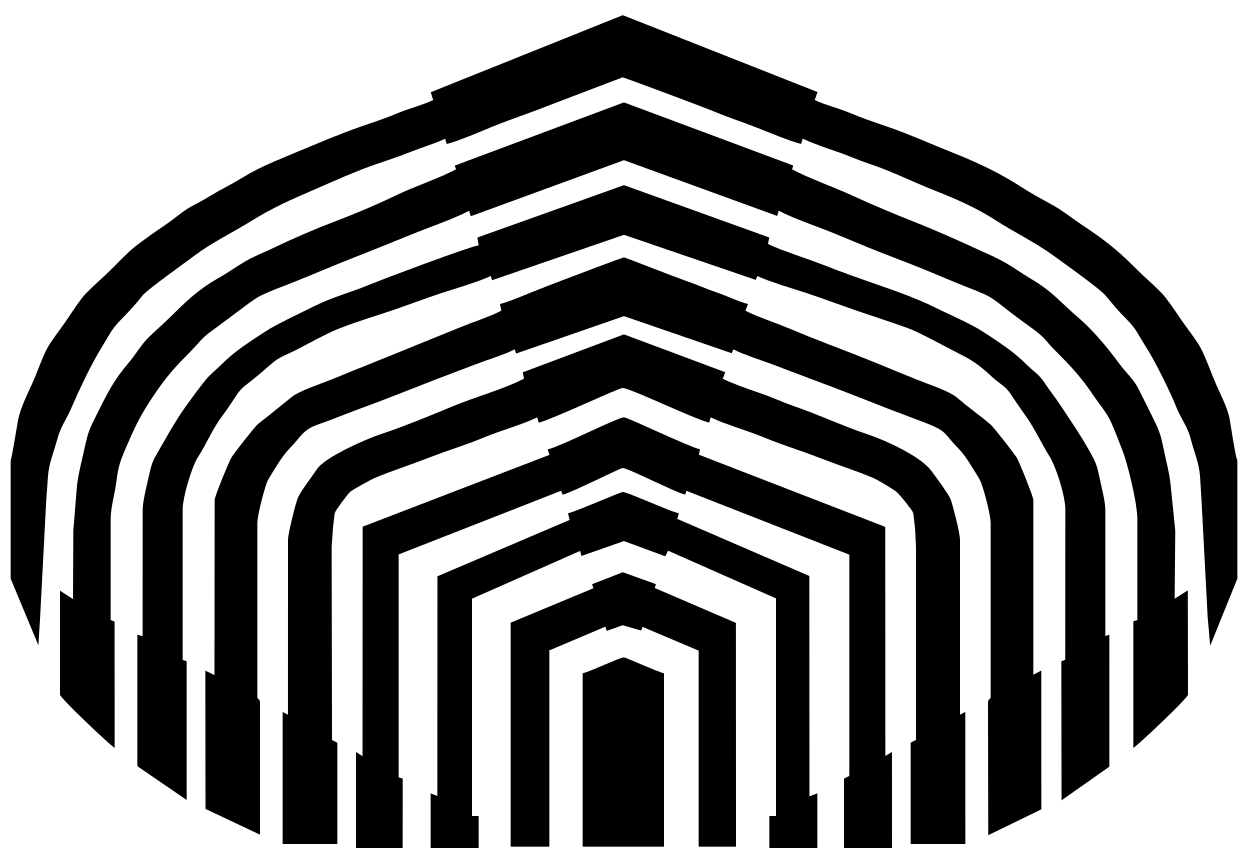
\includegraphics
			[width=.35\marginparwidth]
			{/home/jhonny/git/LaTeX-University/usb-logo.png}\\
		Universidad Simón Bolívar\\
		Caracas, Venezuela\\
		\end{center}
		\end{minipage}
		}
	{
	\Large\headfont
		\MyTitle
	\par
	}
	\smallskip
	\Asignatura\par
	\smallskip
	\@author,\ \today.
	\end{flushleft}
	\vskip 1.5\baselineskip
	}
\makeatother

\usepackage[final]{listings} 
\lstset
{
numbers=left, numberstyle=\tiny\ttfamily, stepnumber=2, numbersep=5pt, 
basicstyle=\ttfamily, 
stringstyle=\ttfamily,
commentstyle=\itshape,
breaklines=true,
postbreak=\mbox{$\hookrightarrow$\enspace},
columns=flexible
}

\usepackage{caption} 
\captionsetup
{
font={rm},
justification=raggedright,
singlelinecheck=false,
skip=3pt
}

\usepackage[explicit]{titlesec}

\titleformat{\section}[hang]
	{\flushleft\headfont}
	{\addfontfeatures{Numbers=Lining}\thesection}
	{1em}
	{\addfontfeatures{LetterSpace=5}\MakeUppercase{#1}}
	[]
\titlespacing*{\section}
	{0em}
	{1.5\baselineskip}
	{.5\baselineskip}
\titleformat{\subsection}
	{\flushleft\sffamily}
	{\addfontfeatures{Numbers=Lining}\thesubsection}
	{.5em}
	{#1}
	[]
\titlespacing*{\subsection}
	{0em}
	{1\baselineskip}
	{1\baselineskip}
\titleformat{\paragraph}[runin]
	{\scshape}
	{}
	{0em}
	{\MakeLowercase{#1}}
	[.]
\titlespacing*{\paragraph}
	{0em}
	{1\baselineskip}
	{5pt}

\let\oldtoc\tableofcontents
\renewcommand
{\tableofcontents}
{\marginpar{\bigskip\oldtoc}}
\usepackage{titletoc}

\titlecontents{section}
	[0em]
	{\vspace{0pt}}
	{\contentsmargin{0pt}}
	{\contentsmargin{0pt}}
	{\contentspage}
	[\vspace{.3em}]
\titlecontents{subsection}
	[1.5em]                              
	{\vspace{0pt}}
	{\contentsmargin{0pt}\small}
	{\contentsmargin{0pt}\small}        
	{\small\contentspage}                 
	[\vspace{.3em}]

\usepackage{fancyhdr}

\renewcommand{\headrulewidth}{0pt}
\setlength{\headheight}{14pt}

\pagestyle{fancy}
\fancyhf{}
\fancyhead
	[L]
	{
	\ifodd\value{page}\MyTitle\else\Asignatura\fi
	}
\fancyhead[R]{\thepage}
\fancypagestyle
	{plain}
	{
	\fancyhead[R]{}
	\fancyhead[L]{}
	\fancyfoot[R]{}%
	\fancyfoot[L]{}
	\fancyfoot[C]{}
	}

\usepackage[thmmarks]{ntheorem}
  % \usepackage[thmmarks]{ntheorem}
  % 	\theoremstyle{plain}
  % 	\theoremindent0cm
  % 	\theorempreskip{0cm}
  % 	\theorempostskip{0cm}
  % 	\theoremheaderfont{\hspace*{\parindent}\upshape}
  % 	\theorembodyfont{\itshape}
  % 	\theoremseparator{.}
  % 	\newtheorem{teo}{Teorema}[section]
  % 	\newtheorem{cor}{Corolario}[teo]
  % 	\newtheorem{prop}{Proposición}[section]
  % 	\newtheorem{lem}{Lema}[section]
  % 	\theoremstyle{nonumberplain}
  % 	\theoremheaderfont{\normalfont}
  % 	\theorembodyfont{\upshape}
  % 	\newtheorem{proof}{Demostración}
  % 	\theoremstyle{plain}
  % 	\theorempreskip{1em}
  % 	\theorempostskip{1em}
  % 	\theoremheaderfont{\upshape}
  % 	\theorempostwork{\noindent}
  % 	\newtheorem{definition}{Definición}[section]

\theoremstyle{plain}
\theorempreskip{\medskipamount}
\theorempostskip{\medskipamount}
\theorembodyfont{\upshape}
\theoremseparator{.}
{
\theoremheaderfont{\itshape}
\newtheorem{definition}{Definición}
}
{
\theoremheaderfont{\scshape}
\newtheorem{theorem}{Teorema}
}


\title{Ejercicios de topología. Evaluación final.}
%\author{Jhonny Lanzuisi, 15\,10759}
\asignatura{Topología 1}

% Algunos macros útiles. Comentar si algo de error.
\newcommand{\Tc}{\mathcal{T}_c}
\newcommand{\Tinf}{\mathcal{T}_\infty}
\renewcommand{\theteo}{\arabic{teo}}
\DeclareMathOperator{\Id}{Id}
\renewcommand{\mathbb}{\symbf}

\let\footnote\null

\begin{document}
	\maketitle
%	\tableofcontents
\noindent Ejercicios del curso de topología 1. Los temas van desde las definiciones básicas hasta espacios conexos.
Estos diez ejercicios representan la evaluación final del curso.

Los diez ejercicios están distribuidos de la siguiente manera:
uno en \S\ref{sec:def}, dos en \S\ref{sec:bas}, dos en \S\ref{sec:fun}, uno en \S\ref{sec:prod}, uno en \S\ref{sec:cociente} y tres en \S\ref{sec:conexo}. Solucion

A veces algunos ejercicios comparten parte de un enunciado, en cuyo caso dicha parte del enunciado aparece una sola vez antes de los ejercicios.
Los párrafos marcados con `\textsc{solución}' corresponden a la solución de cada ejercicio y están colocados inmediatamente después de estos.

\begin{center}
	\rule{4em}{1pt}
\end{center}

\section{Definición de espacio topológico}\label{sec:def}

Sea $X$ un conjunto y sea $\Tc$ el la
colección de todo los conjuntos $U$ de $X$ tales que
$X\setminus U$ es numerable o es todo $X$. Demuestre
que $\Tc$ es una topología sobre $X$.\footnote{Ejercicio tomado del Munkres \cite[\S13, Nº 3]{munkres_topology_2014}}

\paragraph{Solución}

Primero que todo, el conjunto vacío pertenece a $
\Tc $ debido a que $ X\setminus\emptyset=X
$ y $X\in \Tc$ por la definición de
$\Tc$.  También se
tiene que $ X $ es un conjunto abierto puesto que $
X\setminus X=\emptyset $ y el conjunto vacío es finito.

Supongamos que $
\left\{ U_k \right\}$ es una familia de elementos de $
\Tc $.  Entonces\footnote{Este tipo de igualdades se siguen de las leyes de De Morgan}
\[
X\setminus\bigcup U_k= \bigcap (X\setminus U_k).
\]
Pero el lado derecho de la igualdad es numerable\footnote{Véase el Teorema~\ref{teo:interConNum}} puesto
que estas intersecciones son subconjuntos de todos los
$ X\setminus U_k $ y estos últimos son numerables.

Supongamos ahora que $ \left\{ U_1,\dots,U_n \right\} $
son una cantidad finita de elementos de $
\Tc. $ Entonces
\[
X\setminus\bigcap_{i=1}^{n}U_i =
\bigcup_{i=1}^{n} X\setminus U_i.
\]
Donde el lado derecho de la igualdad es numerable pues
la unión de conjuntos numerables es numerable\footnote{Véase el teorema \ref{teo:unionConNum}}.

Hemos visto que las uniones arbitrarias y las
intersecciones finitas de elementos de $\Tc$
pertenecen nuevamente a $\Tc$, esto es, que
$\Tc$ es una topología sobre $X$.

\section{Base de una topología y relaciones de orden}\label{sec:bas}

Sea $X$ un conjunto ordenado parcialmente. Sean $U_L(x)=\left\{ y\mid y\prec x \right\}$ y
$U_R(x)=\left\{ y\mid x\prec y \right\}$, con $x,y$ pertenecientes a $X$.\footnote{Ejercicio tomado del Dugundji \cite[Cap. 3, \S3, Nº 6]{dugundji_topology_1987}}

\subsection{Bases}\label{sec:bases}
Demuestre que las familias $\left\{ U_L(x) \right\}$, $\left\{ U_R(x) \right\}$ son bases de dos topologías
$\mathcal{T}_L$ y $\mathcal{T}_R$, respectivamente, sobre $X$.
Demuestre también que $G$ esta en $\mathcal{T}_L$ si, y solo si, se cumple que 
\[
x\in G\implies U_L(x)\subset G.
\]
Demuestre que en $\mathcal{T}_L$ las intersecciones arbitrarias de conjuntos abiertos dan conjuntos abiertos.

\paragraph{Solución}
Primero veamos que las familias $\left\{ U_L(x) \right\}$, $\left\{ U_R(x) \right\}$
cubren el conjunto $X$. Esto no es muy complicado puesto que, para todo $x\in X$,
los conjuntos $ U_L(x) $ y $ U_R(x) $ contienen a $x$ 
(debido a la reflexividad de $\prec$) de donde se sigue que $X$ puede escribirse
como la unión de los $U_L(x)$ o como unión de los $U_R(x)$.

Tomemos ahora un elemento $y_1$ en $U_L(x_1)\cap U_L(x_2)$, donde
$x_1,x_2$ son elementos de $X$. Entonces
\[
y_1\in U_L(y_1),
\]
por la misma razón que antes, y
\[
U_L(y_1)\subset U_L(x_1)\cap U_L(x_2)
\]
puesto que si tomamos un $y\in U_L(y_1)$ entonces $y\prec y_1$, pero como
$y_1\prec x_1$ y $y_1\prec x_2$, se tiene que $y\prec x_1$ y $y\prec x_2$ por
transitividad. Hemos descubierto que para todo elemento en la intersección de dos $U_L$
podemos conseguir otro conjunto $U_L$ tal que contiene a dicho elemento y esta contenido en la
intersección, es decir, que la familia $\left\{ U_L(x) \right\}$ forma una base para una topología
sobre $X$ por el teorema~\ref{base1}. Esta topología es $\mathcal{T}_L$.

Un argumento análogo al anterior nos da como resultado que la familia $\left\{ U_R(x) \right\}$ también es
base de una topología sobre $X$, y esta topología es $\mathcal{T}_R$.

Supongamos que $G$ pertenece a $\mathcal{T}_L$, entonces $G$ se escribe como una unión arbitraria
de elementos básicos, es decir, 
\begin{align}
	G = \bigcup_\alpha U_L(x_\alpha).\label{eq1}
\end{align}
Si tomamos un $x\in G$ se sigue que $x$ debe pertenecer a alguno de los $U_L(x_\alpha)$. Como $x$ pertenece
a este elemento básico se tiene que $x\prec x_\alpha$ pero entonces, por definición de los $U_L$,
\[
U_L(x)\subset U_L(x_\alpha)
\]
y por la igualdad en~\ref{eq1},
\[
U_L(x)\subset U_L(x_\alpha)\subset G
\]
de donde se tiene, claramente, que $U_L(x)\subset G$.

Supongamos ahora que para cada $x\in G$ se cumple que
\[
x\in G\implies U_L(x)\subset G.
\]
Pero como $U_L(x)$ es un elemento de la base de $\mathcal{T}_L$, la implicación anterior
da de forma inmediata, por el teorema~\ref{base2}, que $G\in\mathcal{T}_L$.

Sea $\mathcal{A}=\left\{ A_\alpha\mid\alpha\in\mathscr{A} \right\}$ una familia de conjuntos abiertos
de $\mathcal{T}_L$, y consideremos la intersección
\[
\bigcap\mathcal{A}.
\]

Si tomamos un $x\in\cap\mathcal{A}$ entonces $x$ pertenece a todos los $A_\alpha$. Como estos conjuntos
$A_\alpha$ son abiertos se sigue, por la parte anterior, que $U_L(x)$ esta contenido en todos
los $A_\alpha$. Pero esto es lo mismo que decir que
\[
U_L(x)\subset\bigcap\mathcal{A},
\]
y, nuevamente por la parte anterior, se tiene que $\cap\mathcal{A}$ es un conjunto abierto.

\subsection{Comparación de topologías}
Demuestre que la topología discreta es la única mas fina que $\mathcal{T}_L$ y $\mathcal{T}_R$. Además las topologías $\mathcal{T}_L$ y $\mathcal{T}_R$ no son comparables.

\paragraph{Solución}
Sea $\mathcal{T}$ una topología sobre $X$ tal que
\begin{align}\label{eq2}
	\mathcal{T}_L\subset\mathcal{T}\quad\text{y}\quad\mathcal{T}_R\subset\mathcal{T}.
\end{align}
Sabemos que al menos una tal $\mathcal{T}$ existe: la topología discreta, a la que llamaremos $\mathcal{D}$, por lo que
tiene sentido preguntarse si existe otra topología con esta propiedad.

Veamos. Dado cualquier $x\in X$, la topología $\mathcal{T}$ debe cumplir (por~\ref{eq2})
\[
U_L(x)\in\mathcal{T}\quad\text{y}\quad U_R(x)\in\mathcal{T}.
\]

Pero como $\mathcal{T}$ es una topología la intersección $U_L(x)\cap U_R(x)=\left\{ x \right\}$ debe pertenecer también a $\mathcal{T}.$
Entonces todos los conjuntos de la forma $\left\{ x \right\}$ ($x\in X$) pertenecen a $\mathcal{T}$, es decir, $\mathcal{D}\subset\mathcal{T}$.

Pero como $\mathcal{D}$ siempre es la topología mas fina, se tiene también $\mathcal{T}\subset\mathcal{D}$, por lo que
$\mathcal{D}=\mathcal{T}$.

Es decir, $\mathcal{D}$ es la única topología más fina que $\mathcal{T}_L$ y $\mathcal{T}_R$.

Notemos primero que se puede establecer un criterio análogo al dado en \ref{sec:bases}
para caracterizar los conjuntos abiertos de $\mathcal{T}_R$, y la demostración de este hecho
es muy parecida a la que esta en \ref{sec:bases}.

Tomemos dos elementos $x_1,x_2$ de $X$ tales que $x_1\prec x_2$. Entonces el conjunto $U_L(x_1)$, que
es abierto en $\mathcal{T}_L$, \emph{no contiene} a ningún elemento $y$ que suceda a $x_1$ (por ejemplo,
no contiene a $x_2$) por lo que $U_R(x_1)\not\subset U_L(x_1)$ y por lo tanto $U_L(x_1)$ no es abierto
en $\mathcal{T}_R$. Un ejemplo análogo nos dará un conjunto abierto en $\mathcal{T}_R$ que no es abierto
en $\mathcal{T}_L$. Entonces se tiene que $\mathcal{T}_L\not\subset\mathcal{T}_R$ y $\mathcal{T}_R\not\subset\mathcal{T}_L$.

\section{Funciones. Continuidad e inclusiones.}\label{sec:fun}

\subsection{Continuidad}

Sean $X$ y $Z$ dos espacios topológicos. Si $Y\subset Z$ y $f\colon X\to Y$, entonces $f$ es continua como una función de $X$ a $Y$ si, y solo si, $f$ es continua como una función de $X$ a $Z$.%\footnote{Ejercicio tomado del Willard \cite[Nº E7]{willard_general_1970}}

\paragraph{Solución}

Supongamos primero que $f$ es continua como una función de $X$ a $Y$. Tomemos un conjunto abierto $V$ de $Z$. Entonces tenemos que
\[ f^{-1}(V)=f^{-1}(V\cap Y),\]
y, como $V\cap Y$ es un conjunto abierto en Y (en la topología relativa),
la continuidad de $f$ nos da como resultado que $f^{-1}(V)$ es abierto en $X$ y que $f$ es continua como una función de $X$ a $Z$.

Supongamos ahora que la función $f$ es continua como una función de $X$ a $Z$. Tomemos un abierto $U$ de $Y$. Como $Y$ es un subespacio de $Z$ el conjunto $U$ se escribe como $Y\cap V$, con $V$ algún abierto de $Z$.
Se sigue entonces que
\begin{align*}
	f^{-1}(U) &= f^{-1}(Y\cap V)\\
	          &= f^{-1}(Y) \cap f^{-1}(V)\\
	          &= X\cap f^{-1}(V)\\
	          &= f^{-1}(V)
\end{align*}
de donde se sigue que $f^{-1}(U)$ es abierto en $X$ y por lo tanto $f$ es continua como función de $X$ a $Y$.

\subsection{Inclusiones}

Sean $X,Y$ dos conjuntos. Dados $x_0\in X$ y $y_0\in Y$, entonces las funciones $f:X\to X\times Y$ y 
$g: Y\to X\times Y$ definidas por
\[
f(x)=(x,y_0)\quad\text{y}\quad g(y)=(x_0,y)
\]
son \emph{inclusiones}\footnote{Ejercicio tomado del Munkres \cite[\S18, Nº 4]{munkres_topology_2014}.}.

\paragraph{Solución}

La función $f$ es inyectiva puesto que
\[
f(x_1)=f(x_2)
\]
implica
\[
(x_1,y_0)=(x_2,y_0)
\]
y esto, por definición del producto cartesiano, implica
que $x_1=x_2$. Un razonamiento análogo nos dice que la
función $g$ también es inyectiva.

Entonces, si restringimos el rango de $f$ y $g$ a sus
imágenes directas obtenemos dos funciones $f',g'$
biyectivas. Para ver que $f,g$ son inclusiones solo
hace falta ver que $f',g'$ y sus inversas son
continuas.

Para ver que $f'$ es continua, notemos que esta función
se puede escribir de la forma
\[
f'=(\id_X,\gamma),
\]
donde $\id_X$ es la identidad de $X$ y $\gamma:X\to Y$ 
es la función constantemente igual a $y_0$.

Entonces la continuidad de $f'$ se sigue de la
continuidad de estas dos funciones\footnote{Véase el teorema \ref{cont:funccoord}}. Un argumento
análogo sirve para la función $g'$ y por lo tanto
$f',g'$ son ambas continuas.

Al igual que antes, una vez que veamos que $f'^{-1}$ es
continua un argumento completamente análogo nos dará
como resultado que $g'^{-1}$ es continua. Para ver la
continuidad de $f'^{-1}$ notemos que esta función esta
dada, al fijar un $y_0\in Y$, por
\[
f'^{-1}=\pi	
\]
donde $\pi$ es la proyección canónica de $X\times\left\{ y_0 \right\}$
sobre $X$. Entonces la continuidad de $f'^{-1}$ se
sigue de la continuidad de $\pi$\footnote{Véase el teorema~\ref{cont:proy}}.

Tenemos entonces que $f',g'$ y sus inversas son
continuas, por lo que $f,g$ son inclusiones.

\section{Topología producto}\label{sec:prod}

Sean $A$ un conjunto de indices y $X_{\alpha} (\alpha\in A)$ una familia de espacio topológicos.
Demuestre que si los $X_{\alpha}$ son espacios de hausdorff
entonces el producto
\[
\prod_{\alpha\in A} X_{\alpha}
\]
es un espacio de Hausdorff tanto en la topología caja como en la topología producto.\footnote{Ejercicio tomado del Munkres \cite[\S19, Nº 3]{munkres_topology_2014}}

\paragraph{Solución}

Tomemos dos puntos $x,y$ distintos en $\prod X_{\alpha}$. Basta con construir
un entorno de $x$ que no contenga a $y$ (tanto en la topología caja como en la producto)
y el resultado buscado se obtendrá entonces haciendo un argumento simétrico para $y$.

Como $x$ y $y$ son distintos,
existe al menos un índice $\beta$ en $A$ tal que $x_{\beta}\neq y_{\beta}$.
Como $X_{\beta}$ es un espacio de Hausdorff, existe  un entorno $U$
(tanto en la topología producto como en la caja)
en $X_{\beta}$ de $x_{\beta}$ que no intersectan a $y_{\beta}$.

Consideremos la familia de conjuntos $U_\alpha$ dada por
\[
U_{\alpha}=
\begin{cases}
	U &\text{si}\;\alpha=\beta,\\
	X_\alpha &\text{si}\;\alpha\neq \beta.
\end{cases}
\]
Notemos que cada $U_\alpha$ es abierto en $X_\alpha$ y tomemos el producto
\[
W=\prod_{\alpha\in A} U_\alpha.
\]
Evidentemente $W\subset\prod X_{\alpha}$. También, como $x_{\beta}\in U$ 
(por la forma en que se eligió $W$) y $x_\alpha\in X_{\alpha}$ para
$\alpha\neq\beta$, se sigue que $x\in W$. Por ser $W$ un producto
de conjuntos abiertos se sigue que es abierto en la topología
caja, como además todos menos una cantidad finita de los 
$W_\alpha$ son iguales a los $X_\alpha$ se tiene que $W$ también
es abierto en la topología producto.

Entonces, sin importar cual de las dos topologías tomemos (la caja o la producto)
el conjunto $W$ será un entorno del punto $x$. Solo queda por ver que este entorno
no intersecta al punto $y$. Esto último podemos verlo mediante un argumento por
contradicción.

Supongamos que $y\in W$. Entonces se tiene que $y_\alpha\in U_\alpha$ para cada $\alpha\in A$.
Pero esto implica, en particular, que $y_{\beta}\in U$.
Lo cual es una contradicción.

Hemos obtenido entonces que $W$ es un entorno de $x$ que no contiene a $y$.
De manera similar pude construirse un entorno $V$ de $y$ que no contenga a $x$
y queda demostrado que $\prod X_\alpha$ es un espacio de Hausdorff.

\section{Topología cociente}\label{sec:cociente}

Sea $p\colon X\to Y$ una función continua. Demuestre que si existe una función continua $f\colon Y\to X$ tal que $p\circ f$ es igual a la identidad de $Y$, entonces $p$ es una función cociente.

Use el resultado anterior para demostrar que una retracción  $r$ de $X$ en $A$ es una función cociente. Si $A\subset X$ una retracción de $X$ en $A$ es una función continua y sobreyectiva tal que $r(a)=a$ para cada $a\in A$.\footnote{Ejercicio tomado del Munkres \cite[\S22, Nº 2]{munkres_topology_2014}}

\paragraph{Solución}

La función $p$ es continua. Tomemos un conjunto $U$ de $Y$ tal que $p^{-1}(U)$ es abierto en $X$. Entonces
\begin{align*}
	f^{-1}(p^{-1}(U)) &= (p\circ f)^{-1}(U) \\
					  &= \Id_Y^{-1}(U)\\
					  &= \Id_Y(U)\\
					  &= U.
\end{align*}
Como $f$ es continua entonces este conjunto $U$ ha de ser abierto en $Y$, y tenemos como conclusión que $p$ es una función cociente.

La retracción $r$ es una función cociente debido a que, usando la parte anterior, la función de inclusión de $A$ en $X$ toma el papel de la función $f$ en el resultado anterior. Siendo la función de inclusión, como es usual, la función $f\colon A\to X$ definida por $f(a)=a$ para cada $a\in A$.

\section{Espacios conexos}\label{sec:conexo}

Sea $X_{\alpha\in J}$ una familia indexada de espacios conexos. Sea
\[
X=\prod_{\alpha\in J} X_\alpha,
\]
y sea $a=a_\alpha$ un punto fijo de $X$.\footnote{Tomado del Munkres \cite[\S23, Nº 10]{munkres_topology_2014}}

\subsection{Definición espacio conexo}

Dado un subconjunto $K$ de $J$ finito, llamemos $X_K$ al subespacio de $X$ dado por los puntos
$x$ tales que $x_\alpha=a_\alpha$ si $\alpha\not\in K$. Demuestre que $X_K$ es conexo.

\paragraph{Solución}
Sean $\alpha_1,\dots,\alpha_n$ los elementos de $K$, llamemos $P$ al producto $\prod_{\alpha\in K}X_\alpha$,
y consideremos la función 
$f:P\to X_K$ dada, para $x\in P$, por $f(x)=z$ donde
\[
z_\alpha= \begin{cases}
	x_\alpha &\text{si}\; \alpha\in K,\\
	a_\alpha &\text{si}\; \alpha\in J-K.
\end{cases}
\]
Entonces $P$ y $X_K$ son homeomorfos a través de esta $f$. Como $P$ es conexo por
el teorema~\ref{conex:prod}, se tiene que $X_K$ es conexo por el teorema~\ref{conex:contfunct}.

\subsection{Unión de espacios conexos}

Demuestre que la unión $Y$ de todos los $X_K$ es conexa.

\paragraph{Solución}
Sea $Y$ la unión de los $X_K$. Como los elementos de cualquier $X_K$ coinciden con
$a$ en las coordenadas que pertenecen a $K$, se sigue que el punto $a$ esta en
todos los $X_K$ de forma casi inmediata. La conexidad de $Y$ es entonces consecuencia del
teorema~\ref{conex:union}.

\subsection{Clausura y conexidad}

Demuestre que $Y$ es la clausura de $X$ y concluya que $X$ es conexo.

\paragraph{Solución}
Elijamos un punto $(x_\alpha)\in X$. Queremos ver que todo entorno de $(x_\alpha)$ contiene
un punto de $Y$. Elijamos un entorno $U$ de $(x_\alpha)$. Como estamos bajo
la topología producto, este entorno $U$ es un producto de abiertos donde todos
menos una cantidad finita de ellos son iguales a los $X_\alpha$. Sea
$K=\{\alpha_1,\dots,\alpha_n\}$ esta cantidad finita de índices.

Entonces podemos hallar un punto $(y_\alpha)$ que esta en $X_K$ y  en $U$ de la siguiente manera:
hagamos $y_\alpha=a_\alpha$ para $\alpha\notin K$ y para los $\alpha\in K$ tomamos $y_\alpha$
tales que pertenecen a $U_\alpha$, donde los $U_\alpha$ son los términos
del producto, que conforma a $U$, que difieren de los $X_\alpha$.

Luego como $(y_\alpha)\in X_K$ entonces también pertenece a $Y$ y se tiene
que $X$ es la clausura de $Y$.

Por lo que $X$ es conexo por el teorema~\ref{conex:cerrad}. Todo lo anterior en realidad ha demostrado
el siguiente teorema:
\begin{quote}
	En la topología producto, el producto arbitrario de espacios conexos es conexo.	
\end{quote}

\section{Resultados teóricos utilizados}

\begin{quote}
	\small Los resultados provienen principalmente del Munkres \cite{munkres_topology_2014},
	aunque algunos son del Dugundji \cite{dugundji_topology_1987} y el Willard %\cite{willard_general_1970}.
\end{quote}

\begin{teo}\label{teo:interConNum}
	La intersección de conjuntos numerables es numerable.
\end{teo}

\begin{teo}\label{teo:unionConNum}
	La unión de conjuntos numerables es nuevamente numerable.
\end{teo}

\begin{teo}\label{base1}
	Sea $\mathcal{B}=\left\{ U_\alpha \mid \alpha\in \mathscr{M} \right\}$ una familia de subconjuntos de $X$
	que cubre a $X$ y satisface la siguiente condición:
	\begin{itemize}
		\item 	Para cada $(\alpha,\beta)\in\mathscr{M}\times\mathscr{M}$ y cada $x\in U_\alpha\cap U_\beta$,
		existe un $U_\gamma$ tal que $x\in U_\gamma\subset U_\alpha\cap U_\beta$.
	\end{itemize}
	
	Entonces el conjunto $\mathcal{T}(\mathcal{B})$ que consiste de $X,\emptyset$ y todas las uniones de miembros
	de $\mathcal{B}$ es una topología sobre $X$, es decir, $\mathcal{B}$ es la base de \emph{alguna}
	topología sobre $X$.
\end{teo}

\begin{teo}\label{base2}
	Sea $\mathcal{B}\subset\mathcal{T}$ una base para la topología $\mathcal{T}$. Entonces un conjunto $A$
	es abierto (es decir, pertenece a $\mathcal{T}$) si, y solo si, para cada $x\in A$ existe un
	$U\in\mathcal{B}$ tal que $x\in U\subset A$.
\end{teo}

\begin{teo}\label{cont:funccoord}
	Las proyecciones sobre la primera y la segunda componente $\pi_1,\pi_2$ ---definidas en el producto cartesiano $X\times Y$--- son funciones continuas.	
\end{teo}

\begin{teo}\label{cont:proy}
	Sea $f:A\to X\times Y$ una función dada, para cada $a\in A$, por
	\[
	f(a)=(f_1(a),f_2(a)).
	\]
	Entonces $f$ es \emph{continua} si, y solo si, las funciones
	\[
	f_1:A\to X\quad\text{y}\quad f_2:A\to Y 
	\]
	son continuas. 
\end{teo}

\begin{teo}\label{conex:contfunct}
	La imagen de un espacio conexo bajo una función continua es conexo
\end{teo}

\begin{teo}\label{conex:prod}
	El producto finito de espacios conexos es conexo.
\end{teo}

\begin{teo}\label{conex:union}
	La unión de una colección de subespacios conexos de un espacio $X$ que tienen un
	punto en común es conexa.
\end{teo}

\begin{teo}\label{conex:cerrad}
	Sea $A$ un subespacio conexo de $X$. Si $A\subset B\subset\bar A$, entonces $B$
	también es conexo.
\end{teo}

\printbibliography[
heading=bibintoc,
title={Referencias bibliográficas}
]
\end{document}
